% !TeX root = ../main.tex

\chapter{Evaluation}\label{chapter:Evaluation}

In order to evaluate the benefit of using the aforementioned feedback mechanisms in regards to the embodiment of feet, a user study was performed. For this user study, a suitable test environment had to be built to showcase these feedback mechanisms.
\newline
During early testing it was found that, in its current state, the remote avatar in the \gls{nrpa} simulation did not manage to follow the local avatar at an acceptable speed. The result was that, even for any reasonable tolerance timer setting, discrepancies would constantly be detected for any limb that moved, due to the remote avatar taking too long to move to the target position, and often overshooting it once it caught up. To get a semblance of intended behaviour, it was necessary to move in slow motion. 
\newline
As the \gls{nrpa} and the \textit{Neurorobotics Unity3D Client} are undergoing constant development, it is assumed that this should work in real time in the future.
\newline
As an alternative, a similarly behaving second avatar with colliders was implemented, taking over the role of the remote avatar, which is connected to the local avatar with spring joints (see Figure\autoref{fig:avatarCollider}). This resulted in behaviour which closely mimics the intended behaviour of the avatar in the \gls{nrpa} simulation, so the findings in this evaluation should be applicable to using the \textit{Neurorobotics Unity3D Client} with a 
\gls{nrpa} instance. Following this, the test environment could be built fully in \textit{Unity}, utilising the built in physics system.
\begin{figure}[h]
    \centering
    \subfloat[Second avatar with colliders attached]{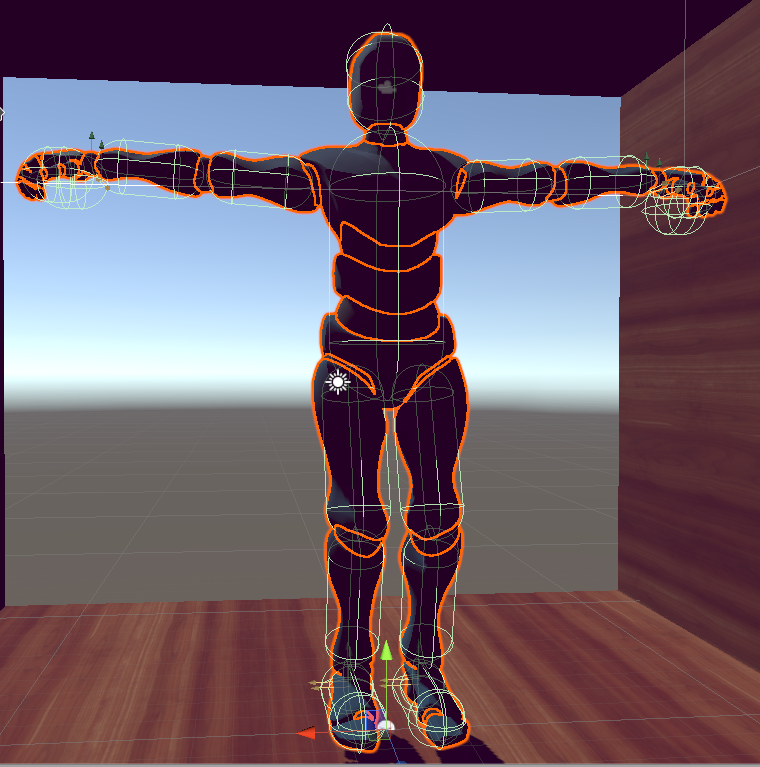
\includegraphics[width=0.45\textwidth]{figures/AvatarCollider}\label{fig:avatarCollider}}
    \hfill
    \subfloat[Plank test environment]{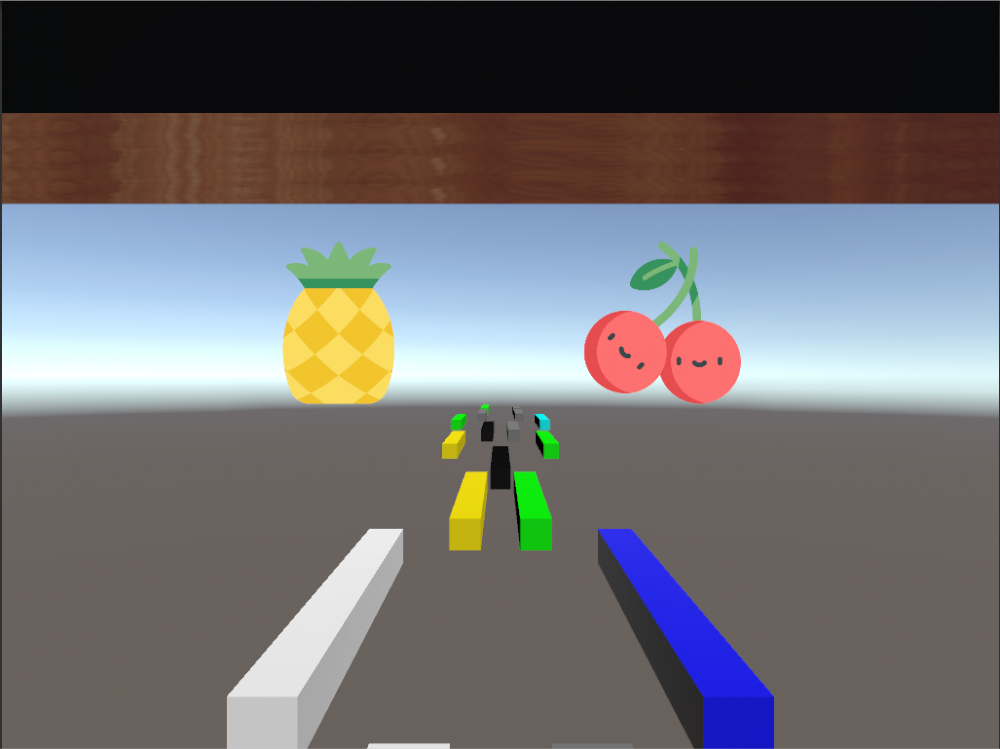
\includegraphics[width=0.45\textwidth]{figures/plankTest}\label{fig:plankTest}}
    \caption{Avatar setup and initial plank test environment}
    \label{fig:avatarAndPlankTest}
\end{figure}

Initially, as a test environment, a little game was implemented, which placed the user in a small hut, with random constellations of planks, endlessly spawned, moving towards him (see Figure\autoref{fig:plankTest}). The idea was that, due to these planks always being in different positions, this would invariably lead to discrepancies at the user's feet, when they collided with him. In order to distract the user from dodging the planks, two canvases displaying changing, random images floated in front of the hut. If a watermelon appeared on the left canvas, the user was to squeeze the controller in his left hand, if it appeared on the right, vice versa. Successfully squeezing the correct controller was rewarded with a little success icon in between the two random images.
\newline
During testing, however, it was found that, when the planks moved fast enough for the user to be hit by them, the discrepancies did not last long enough for any of the feedback mechanisms to be noticed sufficiently, especially when things got hectic. Slowing the planks down, made it too easy to dodge them, which again provided no insight into the usefulness of the feedback mechanisms.
\newline

Another test environment was then created, placing the user in a small room with a protruding wall, behind which is a hole (see \autoref{fig:userStudyTest}). The user is asked to face the yellow wall, and try to move a ball, which is spawned in front of that wall, out of the room, through the hole. When the user walks over to the ball, a platform slides out of the wall and knocks the user's (virtual) feet out from under them, creating a discrepancy at his feet. If the user resolves this discrepancy by moving away from the yellow wall towards his remote feet, the wall will be slid back, and the user can attempt to move the ball out of the room by kicking and shoving it with his feet.
\newline
The toggling of the various effects, as well as the sliding platform and ball spawning is done manually at runtime using the \textit{Unity} editor.
\begin{figure}[h]
    \centering
    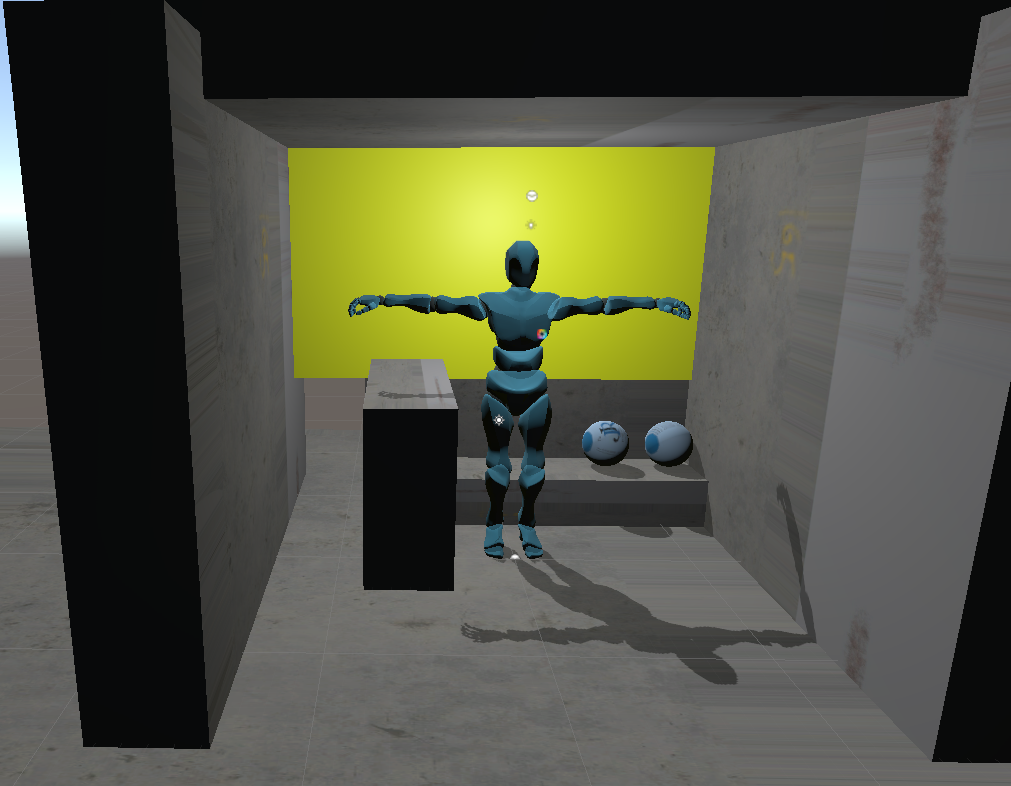
\includegraphics[height=0.3\textheight]{figures/UserStudyBallRoom}
    \caption{Final user study test environment}
    \label{fig:userStudyTest}
\end{figure}


\section{User Study}

For the user study, eight test subjects were recruited during the course of a day with the promise of snacks and drinks for taking part. Of these test subjects, all but one were in the age bracket 18-30. More than half of the test subjects were female, and 75 percent had no prior experience with \gls{vra}.
\newline
The user study had the following procedure for each tested feedback mechanism:
\begin{itemize}        
    \item Set up currently tested feedback mechanism \textbf{X}
    \item Ask subject to face the yellow wall
    \item Spawn a ball
    \item Ask subject to move a ball out of the room
    \item When close enough, slide in the platform to cause a discrepancy
    \item Let subject resolve the discrepancy
    \item Remove platform
    \item Let subject move a ball out of the room with his feet
    \item Ask subject questions and fill out questionnaire with the answers:
    \begin{itemize}
        \item \enquote{How connected to your virtual body did you feel with \textbf{X}?} on a scale from 1 (low connection) to 5 (high connection)
        \item \enquote{How much did \textbf{X} help you notice and correct discrepancies?} on a scale from 1 (hardly) to 5 (a lot)
        \item \enquote{How distracting was \textbf{X}?} on a scale from 1 (hardly) to 5 (very)
    \end{itemize}
    \item Discuss uncertainties about the questions and additional comments by the subject
\end{itemize}
The tested feedback mechanisms for discrepancies at the feet were:
\begin{itemize}
    \item Ghost body only as a baseline
    \item Avatar silhouette visible inside of objects
    \item Line effect
    \item Geiger sound effect
    \item Noise sound effect
    \item Discrepancy indicators
    \item Colour shift effect
    \item Desaturation effect
\end{itemize}
See \autoref{section:feedbackMechanismList} how these work.


\section{Results}
\begin{figure}[h]
    \centering
    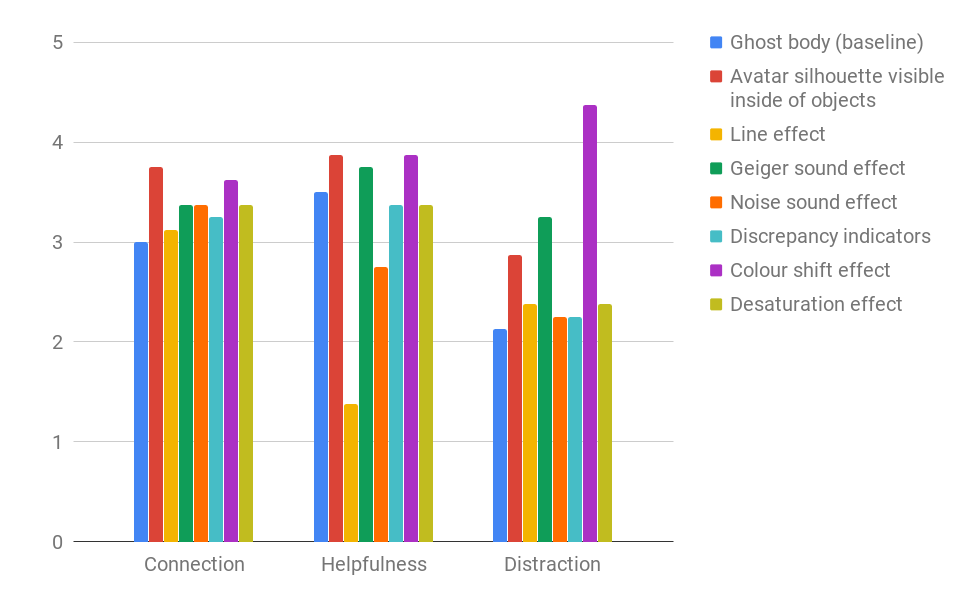
\includegraphics[height=0.4\textheight]{figures/UserStudyAveragedChart}
    \caption{Averaged answers for all tested feedback mechanisms}
    \label{fig:averagedUserStudyChart}
\end{figure}

As can be seen in \autoref{fig:averagedUserStudyChart}, the amount of connection to the virtual body felt by the test subjects (indicating their \gls{soea}) did not differ by a large margin from the baseline of just having a ghost body in a similar pose to their real body. The reason for this is most likely that the ghost body is active in all effects, and already provides a large benefit to \gls{soea}. A notable exception is having the silhouette of this ghost body visible inside of objects, which almost increased the connection by a full point. The least impactful addition was the line effect, with barely any increase over the baseline.
\newline
Looking at the helpfulness of these effects in noticing and correcting discrepancies, a much larger variance between effects can be seen. The ghost body baseline already has a fairly good rating, which is increased again by seeing it inside of objects. Of the two auditory feedback mechanisms, the Geiger sound effect is rated significantly more helpful. The colour shift effect is also rated comparatively high. The least helpful by a large margin is the line effect, which is most likely because the lines are hard to see down by the feet, and often are occluded by the user's body.
\newline
When considering how distracting (as in having a negative impact on \gls{immersiongl}) these feedback mechanisms are, it can be seen that the most helpful effects are simultaneously the most distracting. This is unfortunate, but understandable, as the noise sound effect, desaturation effect, and line effect can be too subtle to prompt the user to take action, whereas the colour shift effect, Geiger sound effect and the avatar silhouette visible inside of objects are a lot more obvious. An exception to this pattern is the discrepancy indicators, which rate fairly high on helpfulness, but low on distraction. This makes sense when only looking at discrepancies at the feet, since this effect is good for alerting the user to discrepancies which are out of view, as feet usually are.
\newline

It was suggested by a test subject that the colour shift effect could be modified to tint the entire view red as opposed to shifting all colours, under the assumption that most people would understand red as a warning sign. Another suggestion was to somehow make the appearance of the avatar silhouette in objects less jarring, in order to make it feel more part of the world. The noise sound effect was felt likely to blend in to background noise. Most subjects suggested combining multiple effects.

The conclusion drawn is that most feedback mechanisms worked as intended for discrepancies at the feet, apart from the line effect, which in Haudenschild's work also did not offer much benefit for discrepancies at the hands \autocite[p. ~32]{JohnnyVEThesis}.  
